\documentclass[a4paper]{article}
\usepackage{float}
\usepackage{tikz}
\usepackage{fancyvrb}
\usepackage{verbatim}
\usepackage{color,graphics}
\usepackage{hyperref}
\hypersetup{pdftex,colorlinks}
\usepackage{titlesec}
\usepackage{titletoc}
\usepackage{enumitem}
\usepackage{geometry}
\date{2021-12-20}
\title{Interlock}
\author{Interlock Team}
\hfuzz=50.02pt
\begin{document}
\maketitle
\tableofcontents

\pagebreak


\begin{abstract}
The web requires \emph{trust} between many participants to reach its
fullest potential. However, we (as in humanity) have centralized the
trust-rating function to a handful of gatekeepers, who themselves have
questionable credibility and competence. We propose a solution that uses
blockchain and other technologies to increase security, privacy, and
trust and bypasses those gatekeepers.
\end{abstract}

\section{Introduction}
The thing about these kinds of papers --- whitepapers --- is that they
are supposed to be confident, authoritative, and seductive. Why, we hear
you ask? Because stringing together words that create an impression of
authoritative and seductive confidence is what often convinces people to
buy whatever it is you are selling. Everybody wants to invest in the
impossible-to-miss certain-to-win solution to some problem that the
market has. We have gone through a lot of whitepapers written with the
confidence and certainty of a devout missionary seeking converts and, of
course, donors. We are not going to do that to you.

Make no mistake, we \emph{are} trying to \emph{convince} you of the
merits of our vision and idea --- we just have no interest in \emph{
hypnotizing} you into agreeing with us. If you believe that the Web is
not living up to its founding promises --- and you want to change this
--- then please read on.

\section{The Problem}
\subsection{History}
The writers of this paper, fellow traveler, are old enough to remember
the following: napster, gnutella, bit-torrent, Usenet, slashdot, RSS
Feeds, Tor, Google before it became evil, and Open Source before it
became cool. We remember an internet where nobody knew that you were a
dog --- and, more importantly, nobody cared. We remember when being
social on the internet meant that you had a blog, read (and shared files
on) USENET, and participated in Slashdot discussions and flame-wars as
an ``Anonymous Coward''. We remember that being informed meant that you
used Google Reader (RIP) to read RSS feeds which were absolutely
everywhere. And if you \emph{really} wanted to stick it to The Man,
you installed Linux on your second-hand beige-box and Firefox on your
folks' Windows computer --- we still have vivid memories and strong
feelings about MSFT, and quite a bit of residual PTSD and mental
scar-tissue. But, somewhere along the way, the internet took a turn. Now
people use Facebook instead of USENET, Twitter instead of RSS, and
Netflix, YouTube, and Spotify instead of BitTorrent. Also USENET,
Slashdot, and friends are all ghost-towns --- while their nearest
equivalents have been overrun by trolls, cat-pictures, memes,
advertisers, and cybercriminals. Oh, and Microsoft is an increasingly
popular and increasingly open-source company --- which is as
inconceivable as Ghengis Khan becoming an exemplary Red Cross volunteer.


Clearly, there has been a pendulum swing from a decentralized and
democratic internet to one that is significantly more centralized and
autocratic. A significant driver of this centralization has been the
insight that the majority of people are busy enough that they will give
up control for convenience --- especially if that convenience has a
price-tag approaching \emph{zero}. With the increase in convenience,
things like web-pages and blogs could be created by people who did not
know how to program or administer computers. Even if you did have this
skill-set, chances are you would apply it to a \emph{virtual} computer
in the \emph{cloud} rather than a physical one in your closet. This
centralization of computing was not sinister or evil --- far from it ---
but it was, rather paradoxically, a leap towards making the web
accessible and useful to more people than ever before. In other words,
centralization \emph{did} democratize \emph{participation} in the
web, but it came at the expense of freedom, control, and privacy. The
web that you see today, is the web that Google wants you to see when you
use their search, that Facebook, Twitter, and Instagram want you to see
when you scroll through ``your'' feed. And what they want you to see, is
whatever will make you re-share the content or click on an
advertisement. You are, in effect, plugged into The Matrix --- the
entire cyberpunk oeuvre is not merely dystopic fiction, it is part
prophesy and part warning.

Maybe you are thinking, that does not sound so bad --- maybe we \emph{
have} to sacrifice freedom, control, and privacy to democratize
participation in the web. Maybe. Maybe not. Maybe that is \emph{exactly
} what the feudal Serfs were thinking while they were working the fields
of their lords --- maybe we have to sacrifice control over our bodies,
our labor, and the (literal) fruits of that labor to democratize
participation in agriculture. After all, what is the alternative?
Starvation?

We sympathize, fellow traveler. We sympathize with you, because it is a
perfectly reasonable question to ask. Yes, being excluded and isolated
from the means of production of our era, is infinitely worse than having
our every action tracked, classified, and monetized. But unlike the
quarries, mines, farms, plantations, factories, and refineries of
previous eras --- which all required capital to establish and maintain
and upgrade --- the means of production of \emph{our} era is, well,
\textbf{us}.

Do you post on reddit? \emph{You} are creating the value, \emph{they}
are capturing it. Do you make videos for YouTube? \emph{You} are
creating the value, \emph{they} are capturing it. Do you create
content for OnlyFans? \emph{You} are creating the value, \emph{they}
are capturing it.

\emph{They} conceive of a world where they data-mine --- yes, the
exploitative nature of their business models is even reflected in their
\emph{jargon} --- everything we do, turn that data into money, and
\emph{we} get (basically imaginary) shares, retweets, mentions, likes,
so-called-friends, and so-called-followers. They have even removed
negative actions such as dislikes for fear that it will drive users ---
another revealing bit of jargon --- away. Their mission is to keep us
happy and cheerful while we (happily and cheerfully) make them money.
You know who also does this? Farmers. What does that make \emph{us}?
Livestock. Are you tired of being milked yet?

\subsection{It Gets Worse}
The previous section was a little bleak --- we will give you that. But
--- as you can probably surmise from this section's title --- this paper
is going to get bleaker before it gets brighter.

If the end of the previous section has you feeling like you have been
conned, like you are --- sooner or later --- going to be the eventual
victim of an unsustainable and tenuous pyramid scheme, well, that was
our intent. To be clear, we are not trying to scare you with ghost
stories. We \emph{wish} these were just ghost stories --- the
exaggerations of a handful of nerds, hackers, and cypherpunks trying to
shock you into listening. But the pyramid is built on a shaky foundation
and the dangers are real.

How could it get worse? Well, in addition to being exploited, and
metaphorically robbed, by the feudal lords of the internet, you are also
being exploited, and \emph{literally} robbed, by the scammers and
criminals that have a growing presence on the internet. We have a
multitude of delightful statistics that back up this claim. The areas of
cybercrime, fraud, and identity-theft are so ripe and pregnant with
opportunities that even nation-states are eager to get in on it --- and
they are not even trying to conceal their involvment. Yes, they give
\emph{zero} fucks, because they are confident that the majority of the
populace is too distracted and too impoverished to actually --- in the
words of Morpheus --- \emph{wake up}.

The obvious question is, why are there so many scammers and
cybercriminals. What is there to steal? Is it worth the risk? What are
the risks? Well, the modern cybercriminal is not like a bank-robber or
hostage-taker. The bank-robber or hostage-taker uses coercion and
intimidation to steal money. The modern cybercriminal is more like the
mythical japanese creature \emph{noppera-bo}. This creature is a
faceless ghost that steals the faces of humans. Cybercrime is about
stealing people's faces and using them as masks --- it is about \emph{
deception} more than it is about coercion or violence. The faces in
this metaphor are usually authentication-credentials that may lead the
criminal to their ultimate goal, currency, crypto or otherwise.

And that is just the most obvious form of theft; material theft. Once
business, politics, and religion enter the equation, lines and
categories start to get blurry very fast. For example, can \emph{truth
} be stolen? If so, does that make a flat-earther a criminal? What about
the corporate marketing department that uses flawed benchmarking
methodologies to convince you that their product is superior to the
competition? What about alternative or traditional medicine books? What
about the \emph{hundreds} of pseudo-historical, pseudo-scientific, and
pseudo-sociological narratives that are weaved every election cycle to
convince people that their neighbors and fellow citizens are the cause
of their anguish --- rather than the massive institutions, corporations,
and beaurocracies that have every incentive to profit from and
perpetrate anguish and tragedy across continents and across generations
(you do not have to look further than McDonalds and Phillip-Morris)?

The point is, the truth is very important, but it can be hard to pin
down. Very few things can be considered absolute truths. The web ---
under its current commercialized and oligarchic stewardship ---
perpetuates, exacerbates, and profits from, vanity, greed, delusion,
ignorance, envy, hatred, and outrage. Instead, it should give users the
tools to better understand themselves, human nature, and our
connectedness to all things --- an ancient idea that is in fact more
relevant to the modern world than it ever was to the ancient world.

Criminals and tech corporations both see the internet-user as something
to be exploited. The former seeks to attack and corrupt the state of
your bank account, while the latter seeks to attack and corrupt your
state of mind. You will find it easy, even effortless, to be angry with
the former, but you may find it difficult to be angry with the latter.
You cannot be angry with the tobacco company for selling you exactly
what you asked for.

\subsection{Identity, Trust, Belief}
Before 1971, if you held a dollar in your hand and examined what was
written on it, you would see ``Exchangeable for Gold''. After 1971, it
would only say ``In God We Trust''. We believed in the dollar because we
believed in gold --- now we believe in the dollar because we believe in
the dollar. This is what some historians would call a revolution, others
would call it a \emph{paradigm shift}. Paradigm shifts, and for that
matter paradigms themselves, are --- and please do not mistake this for
belittlement, quite the opposite in fact --- entirely \emph{imaginary
}. You cannot measure or touch a paradigm. A paradigm does not emit heat
or have mass. Yet paradigms have been the organizing principle of
society since humanity learned how to speak and write things down. A
paradigm is a shared hallucination.

Every paradigm contains the seeds of its own destruction. The bible was
the first book that was mass-printed --- shortly after that the catholic
church lost half of its believers to the various protestant
denominations. The feudal and heriditary paradigms of Europe were eroded
and overthrown by the steady growth of capitalism. The industrial
capitalist paradigm had (after the Great Depression) given birth to both
fascism and communism. And the surviving contenders of the
Second World War, created the Cold War (i.e. bipolar) paradigm. This
paradigm collapsed into one of globalisation and informationalism.
Trading new gods for old.

Trust, just like a paradigm, is powered by \emph{belief}. You cross
the street with minimal anxiety because you trust the drivers to be
sober enough to obey the traffic laws (also another good example of a
paradigm). You use the same two passwords on every site because you
trust that the programmers that made the site have a minimal level of
technical competence and a minimal regard for your security and privacy.
Some Runescape-playing twelve-year-old kid drops all their hard-earned
loot in front of another player and presses \verb|Alt-F4| because the
other player told them it was a glitch that would duplicate all of the
items in their inventory --- that kid \emph{trusted} someone who was
\emph{untrustworthy}, and learned a \emph{painful} but \emph{
important} lesson about \emph{trust}. The internet is basically like
that Runescape example. The entire system depends on trust to get
anything done, but there are too many people and you cannot trust them
blindly. What to do? Well, we did what we have always done, we created
institutions (i.e. social networks and banks) and placed our \emph{
trust} and our \emph{faith} in \emph{them}. It sounds perfectly
reasonable, doesn't it? Sure. But such institutions are powered by
people, and the people --- just like criminals and liars --- have to
respond to market-pressures. We used to \emph{trust} our
credit-rating-agencies to tell us which financial entities were \emph{
creditworthy} --- and then we had an economic \emph{meltdown} in 2008
that destroyed the \emph{trustworthiness} of those institutions
themselves. Centralizing trust in a handful of institutions will work in
a pinch but it could eventually, and without warning, fail --- every
paradigm contains the seeds of its own destruction.

\section{The Internet's Paradigm}
\subsection{Status Quo}
The internet, and especially the Web, are either the result or cause ---
hard to tell really --- of a paradigm shift. The mass on-lining of
humanity has shifted the power (i.e. the value or economic surplus) from
the previous power-holders (i.e. the mass media, the industry, the
publishers, etc). Think about it, more people watched the Fortnite
tournament than actual sporting events. In fact, viewership of the
\emph{Olympics} has started declining towards the end of the last
decade --- after a half century of \emph{growing} viewership. Book
stores are no longer mainstream, and the internet's pre-eminent book
store has evolved into a titanic giant that sells \emph{everything}
and delivers it to your residence within 2 days --- and they also
collect rent for roughly \emph{one third} of all computation and
storage that is provisioned on a Cloud. A ride-sharing company has
displaced local taxi-cab companies \emph{in the entire world} --- not
merely in a city or a state or a nation. Video rental stores are few and
far between, but the internet's pre-eminent video rental store, Netflix,
has emerged as a formidable cultural force spending tens of billions of
dollars per year producing original and highly regarded, or at least
highly viewed, films and television series.

This is how paradigm shifts work. Companies try to build modest
businesses in the not-too-contested corner of the marketplace. The
paradigm starts shifting in their favor and they find themselves
capturing more surplus than they know what to do with. They slowly wake
up to the realization that they are at the top of the pyramid --- not by
any strategic brilliance of their own, but rather, because the pyramid
shifted and contorted itself and they happened to be at the right
coordinates at the right time. Western Europe provides an interesting
case study --- the place was a backwater far away from any action until
some adventerous sailors and navigators found sea routes to Asia (that
let them by-pass the Eastern Mediteranean middle-men) and to the
Americas (which would eventually house the worlds most successful and
likely last ever hegemon --- as always, every paradigm contains the
seeds of its own destruction).

\subsection{New Paradigm}
Different people have different ideas about what the next paradigm of
the web is. Web2.0 got us half-way to where we want to be. Its pioneers,
however, could not resist the incentives to maximize the proportion of
the economic surplus that they capture --- even though these Web2.0
business are essentially \emph{built by the users}. And what about
Web3.0? Depends on who you ask. Right now the mainstream thinks that
Web3.0 is the \emph{semantic web} --- a decades-old idea that has
always struggled to gain traction. Meanwhile, an increasing number of
people believe that Web3.0 will center around \emph{blockchain
technologies} --- but they call it \textbf{web3} (we will call it
Web3.0 from now on in this paper).

We believe that the new paradigm for the internet/web is
hyper-decentralization. The web is decentralizing the media and the news
and the publishing industry. The web is decentralizing geography --- two
people a million miles away can interact with each other over video-chat
or VR. The web is decentralizing finance --- even stuffy old banks want
to get in on the DeFi bandwagon. The web is decentralizing the
nation-state --- people often have more in common with globally
dispersed like-minded individuals than their fellow neighbors and
citizens. The web is decentralizing employment --- the number of people
working in the gig-economy and the creator-economy is increasing
(unfortunately this is another example of users creating a surplus that
is captured by online equivalent of a few feudal lords).

We believe that this accelerating trend of hyper-decentralization will
also decentralize the parts of the web that have to do with \emph{trust
}. Right now, the intermediary institutions (i.e. Facebook, Twitter,
Reddit, HN, and so on) that ascribe credibility and trustworthiness do
so in ways that are \emph{opaque}. We do not know \emph{why} certain
tweets appear in our feeds and others do not --- and even if we did,
there is nothing we can do to \emph{customize} our feed (aside from
following/unfollowing various accounts). We can see a Reddit user's
karma-score as well as the score of their individual posts --- which is
slightly less opaque than Hacker News's ranking system --- but we cannot
see \emph{who} up-voted or down-voted that user's posts. In fact, we
have no way of knowing if that karma score has not been accidentally
inflated by a random bit-flip on Reddit's servers --- let alone if it
has been manipulated by an insider or inflated by a voting ring. Similar
logic applies to Twitter and Hacker News. Hacker News has surprisingly
insightful discussions, in spite of its concealment of vote-metadata for
posts, but it is still susceptible to insider manipulation and voting
rings. In short, almost everything you see in the walled-gardens of the
web --- and almost every decision you make --- is determined --- or at
least strongly influenced by --- distant, nameless, and faceless
product-managers and growth-hackers.

These institutions will tend towards fragmentation and decentralization
because, as it stands, they have too much influence over too many
people. If they translate their influence into power (i.e. translating
technical and economic means into political ends), they make other, more
traditional (and better armed), power-holders angry. If they sit idly
and collect profits without intervening in the affairs of their users
(i.e. translating technical means into economic ends), they make those
same power-holders just as angry for not doing enough. All major tech
giants, including amazon, apple, facebook, twitter, and google, are
being taken to court in nearly every major global jurisdiction --- and
this is just the beginning, we can expect cases like these to extend and
multiply over the next decade, creating what is effectively a
power-vacuum that will be filled by smaller, less distracted players.

\section{Economics}
\subsection{Intro: Three Strains of Economic Thought}
Before we continue with our proposed solution, we should probably take a
brief detour into economics-land and express how our proposal fits into
the main frameworks of economics. From the late 1700s up to the
present-day three economic schools of thought have shaped societies
around the world --- namely, the Neoclassical, the Keynesian, and
the Marxian. The Neoclassical school focused on individual freedom and
individual incentives, and rejected any form of state-intervention in
the economy --- in other words they assumed that Utopia was achievable
without Leviathan. After the Great Depression set the
Neoclassical Utopia aflame, the Keynesian school arose and argued that a
Utopia could not be maintained without a Leviathan --- they argued that
the individual was certainly important, but not nearly as important as
the \emph{structure} of the economy. These two views correspond to
microeconomics (i.e. reasoning that individuals ruthlessly pursuing
their own self-interest will create the most desirable outcomes for all
of humanity) and macroeconomics (i.e. reasoning that \emph{tracking}
macroeconomic indicators like GDP, unemployment, inflation, and
interest-rates and \emph{tuning} those macroeconomic variables will
create the most desirable outcomes for all of humanity). Put
differently, one school thinks that individual behavior and actions
\emph{cause} the economy, while the other school thinks that the
economy \emph{causes} individual actions and behavior. To be clear, we
are not taking sides, both points of view are correct they just disagree
about the \emph{relative} value of one component in relation to the
others. And now onto the Marxian school which requires its own
paragraph.

The Marxians are primarily concerned with \emph{the means of production
} --- specifically, what they are, who is the class that owns them, who
is the class that operates them, what are their outputs, what is their
economic surplus, and who captures what proportion of that surplus. They
marvel at the economic efficiency and dynamism unlocked by the
transition from feudalism to capitalism, but they believe that any
arrangement in which the class that operates the means of production but
does not own or control those means is fundementally unjust, and does
not fulfil the (false) promises of Humanism (the philosophy undergirding
both Neoclassical and Keynesian social orders). They also believe that
individuals and economic-structures are always shaping each-other via
never-ending \emph{dialectics} --- in effect, they are \emph{
simultaneously} cause \emph{and} effect. And that is pretty much all
of the Marxian school \emph{that is relevant to this paper} --- there
is a lot of other stuff (i.e. central planning as a suitable alternative
to the market) that is simply not compatible with a globalized
marketplace, nor is it compatible with a trend towards
hyper-decentralization.

We basically agree with all of these theories, and want to use the three
perspectives to construct a globally decentralized network that will
give users freedom, control, privacy, and security.

\subsection{Reputation and Trust}
Trying to eliminate the intermediary institutions that ascribe trust is
a little bit like trying to eliminate the police or trying to eliminate
schools. Obviously policing and schooling are very important and nobody
would ever consider decentralizing them, let alone eliminating them. So
we should ask ourselves, what kind of people have no need for the
police? What kind of people have no need for schools? The answer, fellow
traveler, is people that are \emph{self-policing} and \emph{
self-schooling}. Obviously, such people are very rare, otherwise we
would not need schools and police departments. However, a computer that
is not under the control of any single individual can in fact be used to
implement this kind of flawless self-regulation. If we go back to that
earlier Runescape example from Section 4, the game could have been
programmed to disallow such acts of deception --- whether this makes the
game better is another matter entirely.

What we wish to do is to use the decentralized, history preserving, and
transactional nature of the blockchain to implement an anonymous
trust-network.

Our network associates users with accounts on the blockchain, similar to
how a licence plate is associated with a vehicle --- though \emph{
unlike} a license plate we do not associate the \emph{identity} of
the user with the account.

If Web2.0 was about \emph{websites} and \emph{services}, we believe
that Web3.0 is about \emph{people} and \emph{content} and their
\emph{trustworthiness}.

\section{Why Security}
\subsection{Freedom, Choice, and Privacy}
Security is a difficult problem --- it has \emph{always} been a
difficult problem. Throwing blockchain at the problem won't
automatically fix it. If websites were signed using an account-signature
from a blockchain-powered reputation-network many phishing attacks ---
the most common and most successful kind of attack --- would be a lot
less feasible. However, such a network would \emph{only} protect the
users that have an account on it \emph{from} websites that belong to
\emph{other} users that have an account on it. In effect, we would
have the walled-garden-problem --- only users that were inside the
walled-garden would get protection. This makes the concept no better
than any other walled-garden-approach and would require buy-in from
major players on the internet. In short, a blockchain-based
decentralized reputation-network is not a good starting point for any
entity that is not already very influential (i.e. the existing
gatekeepers like facebook, twitter, and reddit).

Our company, Interlock, has developed an extension --- a fork of uBlock
--- that, in addition to the usual ad-blocking functions, can also
detect whether a website is fraudulent based on very effective, widely
tested, heuristics. When a user opens a webpage that the extension
thinks is fraudulent or untrustworthy, the extension will prevent any
user input to the page and issue a warning in the form of a large red
banner. The extension has already seen use in some large companies that
you have definitely heard of --- and for most of its life it has been
out of the reach of non-corporate users. Our plan is to make this
extension available to \emph{everyone} but to modify it to work with
Interlock Network. When the user installs the extension they can open an
account on the Interlock Network, link it to the extension, and we will
deposite an arbitrary amount of Inter Tokens into their account. As they
use the extension they will get a variable-time and variable-quantity
reward for using it. If the extension mistakenly locks a page a user can
unlock it. If an extension does not lock a page, a user can flag it.
Pages that have been flagged or unlocked are designated as \emph{
grey-area-entities}. Users can also get additional Inter Tokens if they
are willing to \emph{stake} a grey-area-entity. If we determine that a
staked grey-area-entity is actually malicious, the user will lose the
Inter Tokens that have been staked. If, on the other hand, the
grey-area-entity is \emph{not} malicious the user will earn a
percent-reward on the amount staked. This risk/reward arrangement
incentivises users to only stake on sites that have only been mistakenly
flagged by our heuristics or by another user. This staking-information
also helps Interlock refine and sharpen its heuristics. And this is just
the bare-bones, minimum-viable-product-functionality --- in later
releases, users will also be able to flag webpages as \emph{containing
} malicious content (i.e. a comment on reddit or a video on youtube),
effectively crowdsourcing moderation.

\section{KYC}

The \textbf{Know Your Customer} laws are an interesting example of
laws that require establishing the trustworthiness of a customer. In
principle it is basically the same concept as checking whether a website
is legitimate or fraudulent; or whether an account on the
Interlock Network is highly regarded or shunned. Obviously, if all
transactions happened on the Interlock Network --- or on \emph{any}
blockchain --- KYC laws would be trivial to implement. That is one of
the nice side effects of complete transparency. We can combine the data
collected by the Interlock Network with data --- \emph{anonymized} of
course --- that we gather from the extension to help the relevant Web3.0
financial institutions (i.e. namely crypto-exchanges and banks that want
to jump onto the DeFi train) stay in compliance with the KYC
regulations.

\section{Cryptonomics}

\subsection{Interlock Token}

To back our smart-contracts and our token we have chosen the \textbf{
Solana} blockchain technology as our transaction-processing
platform-component and \textbf{Ethereum} as the platform-component on
which we mint the actual tokens. Solana has addressed many of the
outstanding problems found in similar popular blockchains like Ethereum
(i.e. transaction-speed energy-efficiency infinite-smart-contract-loops
etc), and it has excellent documentation and development-stack that we
are quite fond of. Also, building on top of Solana also allows us to
(evetually) add transaction-heavy features to the Interlock Network that
are simply not feasible on any blockchain that does not have cheap
transactions. We had hoped that we would be able to use Ethereum since
it has an enormous ecosystem and is very popular, but its transactions
are thousands of times more expensive than Solana's. We do however
recognize the value of Ethereum's ERC-20 standard and the ability to use
existing wallets and to transact with other people on Ethereum --- so we
are minting the coins on Ethereum but connecting them to Solana using
the Wormhole bridge between these two blockchains. However, if the newer
versions of Ethereum increase the TPS and decrease their
transaction-costs we could see ourselves porting our code over to these
future versions of Ethereum --- assuming that Solana does not supplant
Ethereum in the meantime.

\section{Tokenomics}

\subsection{Token Supply}

In short, we plan to emit \textbf{1 billion} tokens, over an 86-month
period. Here are the first 3 years of emission, divided into half-year
periods.

\begin{table}
\centering
\begin{tabular}{|c|c|c|}
\hline half-year & new-tokens & total-tokens \\ \hline
aug-2022 & 189087820 & 189087820 \\
feb-2023 & 161495487 & 350583307 \\
aug-2023 & 100483712 & 451067019 \\
feb-2024 & 115245098 & 566312117 \\
aug-2024 & 75395270 & 641707387 \\
feb-2025 & 66876750 & 708584137 \\
\hline
\end{tabular}
\end{table}


We also mint new tokens as necessary to meet staking obligations ---
which is only necessary \emph{after} all tokens are emitted, or if all
tokens are held but unused by their owners. Most projects try to
``control'' the price by controlling supply, but we feel that this is a
fool's errand, and that it would be much more robust to \emph{stimulate
demand} for the token by making it \emph{useful} and \emph{desirable
}.

\subsection{Staking and Earning}

Even though we touched on it earlier, we feel it bears repeating under
what circumstances tokens move across the network. There are 4
categories of Interlock Network participants: extension-users,
security-stakers, enterprise-customers, and data-buyers. Extension-Users
earn tokens for sharing data and for flagging/unlocking websites.
Security stakers earn tokens for staking on non-malicious
grey-area-entities (and lose tokens for staking on malicious
grey-area-entities). Enterprise-Customers can buy and stake tokens for
licensing discounts. Data-Buyers can buy and stake tokens for data
discounts. Visual learners may appreciate the diagram below.

\begin{figure}
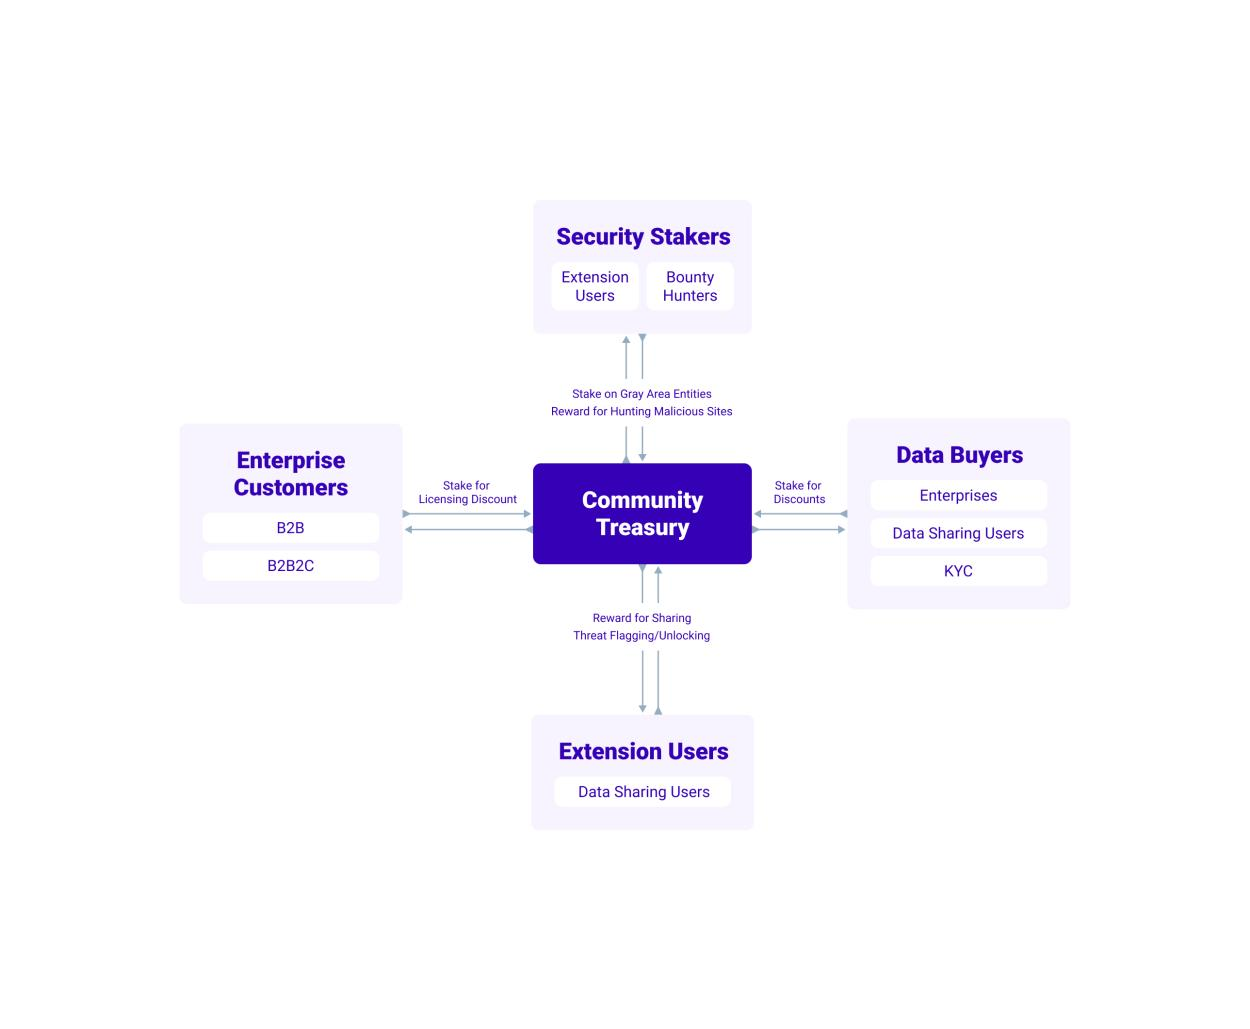
\includegraphics[width=\linewidth]{../../imgs/diagram_light.jpg}
\end{figure}


\subsection{Investing and Governance}

We are evaluating different governance models. Stay tuned.

\section{Technical Contributions}

Regarding technical contribution we will follow an RFD/RFC model where
project design documents are proposed and discussed on various community
channels (i.e. github, discord, and discourse). If the project and
community get large enough we will likely adopt a governance model akin
to Rust's. We do not require separete personal and developer accounts,
but we also do not require the same account. Keeping with the theme of
privacy and anonymity a developer can have as many accounts as they want
and the project/community would have no way of knowing --- which is
\emph{already} the situation in the real world (i.e. one can make as
many github accounts as they want). Voting is consensus-driven ---
proposals require unanimous approval. Unanimous consensus is meant to
eliminate the competitive nature of voting --- all disagreements should
be resolved at the \emph{discussion} phase before a proposal comes to
a vote. We believe that there are very few \emph{true} and \emph{
unresolvable} contradictions in engineering. Proposals can be
resubmitted for voting.

\section{What's Next}

\subsection{security industry and interlock}

We are currently migrating this content from the original whitepaper,
check back later.

\subsection{ecosystem and frictions}

We are currently migrating this content from the original whitepaper,
check back later.

\subsection{phishing statistics}

We are currently migrating this content from the original whitepaper,
check back later.
\end{document}

